\section{Introduction}\seclabel{intro}
Multiple instance learning is a supervised learning scenario first proposed by \citet{dietterich1997solving}.
In multiple instance learning, examples are multi sets of instances, called bags, and each bag is assigned a class label.
It is assumed that each instance has a true label, defined by an underlying concept. The label of a bag is positive, if and only if one of
the instances it contains is labeled positive. The true label of instances is assumed to be unobserved by the learner who only has access to bag labels.

In the original formulation of multiple instance learning, the goal of the learner
was to predict the label of bags. Some recent works also aim at predicting
the label of individual instances, a much harder problem.
This can be viewed as learning an instance-level classifier using a form of weak supervision.

Learning to predict instance labels has been attempted in some recent work~\citep{liconvex2010,zhang2002dd}
but there has been very little theoretical study when and to which extend this is possible.
In this work, we explore which assumptions about the distributions of instances and labels
are necessary to learn instance-level classifiers from bag labels only.
We provide bounds on the instance label prediction error based on the
bag label prediction error. The bounds can be used to judge a learner when no
instance labeling exists for training or testing.
%If one is interested in classifying instances, such a bound is very important.
There are two applications that we target:
\begin{description}
\item[Setting 1:] Bag labels for a validation set are known and instance predictions need to be judged.
\item[Setting 2:] Bag labels for a test set can be bound using standard learning theoretic bounds and instance
predictions need to be judged.
\end{description}
The first case is very common in practical settings, where
cross validation is often used to set parameters of a predictor. This is
particularly important in support vector machines (SVMs) which are a popular
learning method for multiple instance problems~\citep{andrews2003support}.
If no instance labels are present for training, it is only possible to
choose parameters to minimize bag prediction error, which might be suboptimal if one
wants to minimize instance label misclassification. 
The bounds can also be used to find the amount of positive instances in positive bags,
known as the witness rate, which is an integral part of established multiple
instance algorithms~\citep{zhang2002dd,liconvex2010}.
The second case can be used to convert established bounds on the bag prediction error
to instance prediction error.

We show that it is possible to bound instance prediction error without
ever observing any instance labels even in fairly unrestricted settings.
To the authors knowledge, this is the first result of this kind.

Detailed proofs of all propositions can be found in the appendix.

\section{Related Work}
The theoretical analysis of multiple instance learning started with \citet{auer1997approximating} and later \citet{blum1998note}.
These works assume that instances are drawn i.i.d.\ from a single distribution over instances. Blum and Kalai showed that in this
setting, if the underlying concept is PAC-learnable in polynomial time, then the multiple instance learning problem is PAC-learnable
in polynomial time. Auer et\,al.\ showed that if there is an algorithm to PAC-learn multiple instance learning with axis-parallel
rectangles that is polynomial in size of the bag and dimension of the instance features, then it is possible to polynomially
PAC-learn DNF-formulars, a problem that is solvable only if $\text{RP}=\text{NP}$.
Recently, \citet{sabato2009homogeneous,DBLP:journals/corr/abs-1107-2021} proved bounds on the VC dimension and
fat shattering dimension of multiple instance learners by the corresponding dimension for a base learner.

All of the results above only consider predicting bag labels. There has been very little theoretical work
on predicting instance labels. In spite of the large amount of research on multiple instance learning algorithms 
(for example \citet{andrews2003support,gaertner2002multi,zhou2009multi,li2009convex,zhang2002dd,mangasarian2008multiple,leistner2010miforests,chen2006miles})
to the authors knowledge, the only quantitative evaluations of predicting
instance labels are by \citet{gehler2007deterministic} and by \citet{liconvex2010}. While these works show promising results,
no analysis of instance label prediction is given.

Sabato et\,al.\ also studied multiple instance learning as a way
to reduce labeling complexity~\citep{sabato2010reducing}.
In the setting of reducing label complexity, the learner creates
the bags itself. The instances can therefore be assumed to be globally i.i.d.\ and
the distribution of labels inside the bags is known a priori.
Under these assumptions, the instance label prediction error is bound using the bag label error.
This result is used to evaluate the sample complexity of learning from bags using empirical risk minimization.
In this work, we generalize some results from \citet{sabato2010reducing} to the setting where the distribution
of instance labels is unknown and to cases where instances inside a bag may be dependent.

\section{Preliminaries}
Throughout this work, $\mathcal{X}$ denotes the space of all instances. Bags are multi sets of instance $X=\{x_1,\dotsc, x_r\}$.
As usual in supervised learning tasks, we assume our training examples ($X_i,Y_i)$ to be i.i.d.\ from an unknown distribution.
We denote the label of an instance $x_i$ by $y_i$ and the label of the bag $X_i$ as $Y_i = \max\{y_j | x_j \in  X_i\}$.
We assume the bag size $r\in \mathbb{N}$ to be constant over all bags in a given problem. This restriction simplifies the treatment
significantly while our results can in great parts be carried over to settings with varying bag sizes.
We consider arbitrary classifiers $h_I\colon \mathcal{X} \rightarrow \{0, 1\}$ with associated bag classifier
$h_B(X) = \max \{h(x_1),\dotsc,h(x_r)\}$.
The goal is to learn a classifier $h$ which minimizes expected instance misclassification, given training bags and bag labels
$X_i$ and $Y_i$.
We do not consider specific hypotheses classes but instead try to bound the expected error of $h$ using the expected error of $h_B$.
During all of this work, we assume that the true instance labels are never observed.
We use the following notation: $p(h_I(x)=0):= h_0$, the negative rate of the classifier,
$p(h_I(x) \neq y) := e_I$, the instance error, and $p(h_B(X) \neq Y) := e_B$, the bag error.

\section{Necessary Assumptions}\seclabel{assumptions}
If we allow instances inside bags and their labels to have arbitrary dependencies, we are trying to find
$y_1,\dotsc,y_r$ maximizing $p(y_1,\dotsc, y_r | x_1, \dotsc, x_r)$. This is a structured 
prediction problem for which there is no hope solving it, given only bag labels.
Therefore, as usual in multiple instance learning, we assume there is an underlying concept for instances,
i.\,e.\ the label of each instance depends only on this instance.
In other words, we assume $p(y_1,\dotsc, y_r | x_1, \dotsc, x_r)=p(y_1|x_1) \cdot p(y_r|x_r)$.

If we allow arbitrary dependencies between the instances $x_i$ in a given bag, there is a simple example 
\citep{sabato2009homogeneous} that shows that learning instance classification is not necessarily possible.
Let $\mathcal{X}$ consist of two
distinct points $x_1$ and $x_2$ with corresponding labels $y_1 = 1$ $y_2 = -1$. If the distribution
of instances inside bags is such that each bag either contains two copies of $x_1$ or both of $x_1$ and $x_2$, then
by predicting all bags as positive, one can obtain a perfect bag classifier, while it is impossible to say anything
about the label of $x_2$.
Therefore, we need to make additional assumptions about the distribution of instances inside bags to enable
predicting instance labels.

\section{Independent Case}\seclabel{iid}
The simplest case in which learning instance prediction is possible is the case when instances are globally i.i.d.,
i.\,e.\ when instances inside a bag are independent of each other. This is a very strong assumption that might be
violated in practical applications. On the other hand, strong results can be proved in this setting.

\begin{theorem}\label{basicthm}
Let all instances be independent. With bags $X$, instances $x$, true labels $y,Y$, $h_I$ any classifier
on instances and $h_B$ the resulting bag classifier, we have
\begin{align*}
    %\eqlabel{iid}
   e_I = h_0 + p(y=0) - 2 \left (\frac{1}{2} ( h_0^r + p(y=0)^r - e_B) \right)^\frac{1}{r}.
\end{align*}
\end{theorem}
This is a (slight) generalization of Theorem 1 in \citet{sabato2010reducing} and serves as a basis for all further bounds. 

In particular:
\begin{corollary}\label{perfect}
If all instances are independent and bag classification is perfect, meaning $e_B=0$, then instance classification is also perfect ($e_I =0$).
\end{corollary}
This is an very interesting result in that if we do not assume independence, this corollary is wrong,
as shown by the example in \Secref{assumptions}.

In practice, $p(y=0)$ is unknown, as we assume a setting where no instance labels are available.
Thus finding a bound independent of $p(y=0)$ is desirable. The following theorem accomplishes this:

\begin{theorem}\label{iidbound}
If $h_0^r  \geq e_B$ and all instances are independent, we have
\begin{align}
    p(h_I(x)\neq y) \leq h_0 - \left ( h_0^r - e_B \right ) ^ \frac{1}{r}
\end{align}
\end{theorem}

This result, which applies to the Setting $2$ from \Secref{intro},
can be used in several ways. First, it can give a general idea about the quality of instance-level
predictions, without assuming any knowledge of the distribution of instance labels. In this inequality,
$h_0$ can simply be read off on training and/or test data. The other quantity, $e_B$ can be
estimated using standard supervised generalization bounds.

If we assume Setting $1$ from \Secref{intro}, where bag labels are known, we can say even more:
\begin{theorem}\label{equality}
Let all instances be independent. Given $p(Y)$, the instance error $e_I$ can be calculated by
\begin{align}
    %\eqlabel{iid}
e_I = h_0 + p(Y=0)^\frac{1}{r} - 2 \left (\frac{1}{2} ( h_0^r + p(Y=0) - e_B) \right)^\frac{1}{r}.
\end{align}
\end{theorem}
If bag labels are given, $p(Y=0)$ and $ e_B$ can simply be estimated from validation data.
This means, in the i.i.d.\ case, instance-level error can simply be calculated from bag label and classifier statistics.

\section{Restricted Dependent Case}
As remarked in \Secref{assumptions}, it is not possible to bound the instance classification error
when allowing arbitrary dependencies between instances. On the other hand, the i.i.d.\ assumption of \Secref{iid}
might be too strong in a practical setting.
Therefore, we propose an assumption that is both very general and allows learning of instance classification:
We assume that each bag has a ``hidden cause'' $Z$, conditioned on which all instances are independent.
More formally, we assume
\begin{align}
    p(x_1,\dotsc,x_r)=\int_Z p(x_1)\cdot \dotsc \cdot p(x_r) dZ.
\end{align}
The intuition behind this assumption is as follows. In the classical case of drug activity prediction~\citep{dietterich1997solving}, a bag corresponds
to a molecule and each instance corresponds to a different geometric configurations. These are certainly not independent.
If one knew the ``true'' geometric characteristics of the molecule, each configuration could be derived from that.

Another popular example of multiple instance learning is image or scene classification~\citep{zhou2007multi,zha2008joint,zhou2009multi}.
In this case, each image
is represented as a collection of interest points or segments.
For the sake of the argument let us assume that interest points or segments correspond to objects.
Again, objects in a scene are not independent. For example, if we know an image contains a chair and a TV set,
it is very unlikely to contain a bus.
On the other hand, if we knew something about the scene, such as ``this is a living room scene'', then the appearance
of certain objects does not tell us much about other objects.

The idea of introducing a hidden cause is similar to the idea of viewing a bag as a manifold and instances as points
sampled on this manifold, as in \citet{ICML2011Babenko_74}.

Conditioned on the hidden cause $Z$ for a given bag, the proof of Theorem~\ref{basicthm} still holds, yielding
\begin{align}\eqlabel{conditioned}
&p(h_I(x) \neq y | Z) =p(h_I(x)=0|Z) + p(y=0|Z)\\
&\textstyle- 2  [\frac{1}{2} ( p(h_I(x)=0|Z)^r + p(y=0|Z)^r\\
& - p(h_B(X) \neq Y|Z)) ]^\frac{1}{r}
\end{align}
Similarly, the idea of Corollary~\ref{perfect} yields:

\begin{corollary}\label{perfect}
If the bag classification is perfect, meaning $e_B=0$, then instance classification is also perfect.
\end{corollary}

While this is a very simple result, is has strong implications. In particular, albeit we generalized our
assumptions significantly, learning instance label prediction is still possible.
As we assume no knowledge of the distribution of the hidden bag variable $Z$ or even about its domain, it is significantly harder
to bound the instance error than in the i.i.d.\ case.
Using Theorem~\ref{iidbound} and taking expected values with respect to $Z$, we obtain
\begin{align}
    & p(h_I(x)\neq y) \\\
    & \leq h_0 - \mathbb{E}_Z \left [\left ( p(h_I(x)=0 | Z)^r - p(h_B(X)\neq Y|Z) \right ) ^ \frac{1}{r} \right ].
\end{align}


\begin{figure}[tbp]
	\begin{center}
		
\includegraphics[height=40mm]{images/gehler_decision_boundary.png}\hspace{5px}
		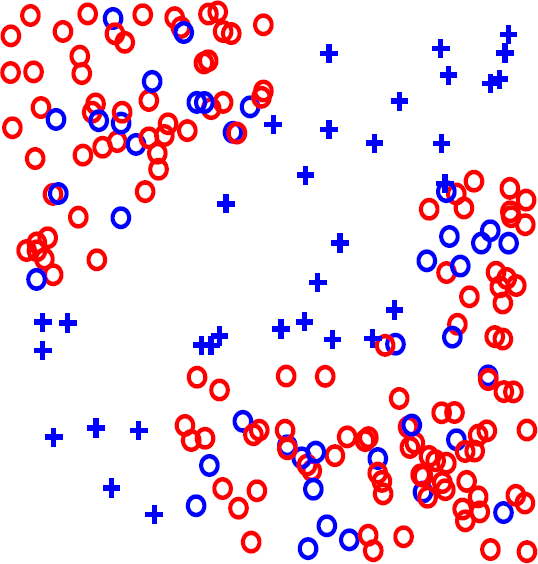
\includegraphics[height=40mm]{images/gehler_instances.png}
	\end{center}
	\caption{Visualization of the dataset from \citet{gehler2007deterministic}. Left: Regions in $\mathbb{R}^2$
    corresponding to negative and positive instances. Right: Training points for 40\% positive rate. Red denotes negative
    bags, blue denotes positive bags. Crosses denote positive instances, circles negative instances.}
	\figlabel{gehler}

\end{figure}
To get a better handle on the behavior of instance errors, it may also be useful to lower-bound $e_I$.
This is possible using Theorem~\ref{basicthm}:

\begin{theorem}\label{lowerbound}
If the instance labels are independent inside a bag given a hidden cause, the instance
error $e_I$ has the following lower bound:
\begin{multline*}
e_I \geq h_0 + p(y=0)\\ 
- 2 \left (\frac{1}{2} (p(h_B(X)=0) + p(Y=0) - e_B) \right)^\frac{1}{r}.
\end{multline*}
\end{theorem}


\section{Experiments}
We evaluate the tightness of our bounds and their utility for finding parameters on the sythetic dataset of \citet{gehler2007deterministic}.
This dataset allows us to vary $p(y=0)$, which is half of the positive rate in positive bags.
A visualization of the dataset, which we refer to as Gehler-org is shown in \Figref{gehler}. In Gehler-org, there are as many positive
as negative bags, 30 of which are commonly used for training and 100 of which are used for testing.
We use 1000 bags for testing, resulting in more stable estimates of errors and bounds.
When generating the dataset, one fixes a rate of positive instances, also known as witness rate, which determines the ratio
of positive instances in a positive bag.

To evaluate our bounds in the i.i.d.\ setting, we have to modify the dataset slightly. We fix bag size at ten instances and generate instances
with a fraction of positive instances of half the witness rate. Then we randomly assign these instances to bags.
This way, the distribution over instances stays the same as in Gehler-org while instances inside bags become independent.
We refer to this dataset as Gehler-iid.
As a multiple instance learning algorithm, we choose SVM-SVR from \citet{liconvex2010}, as a state-of-the-art method that
provides instance predictions. Support vector regression is learned to estimate likelihood ratios of label instances.

\begin{figure}[tbp]
	\begin{center}
		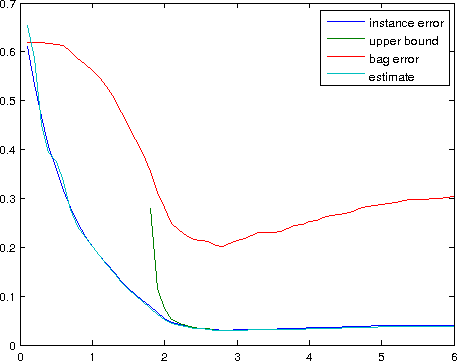
\includegraphics[height=63mm]{images/iid_01.png}
		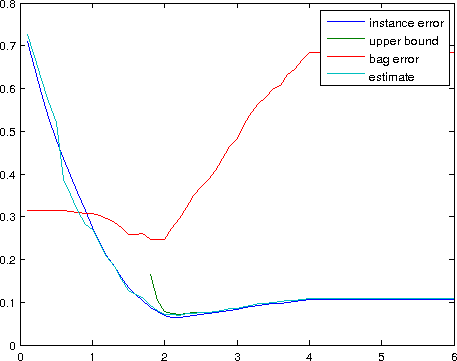
\includegraphics[height=63mm]{images/iid_02.png}
		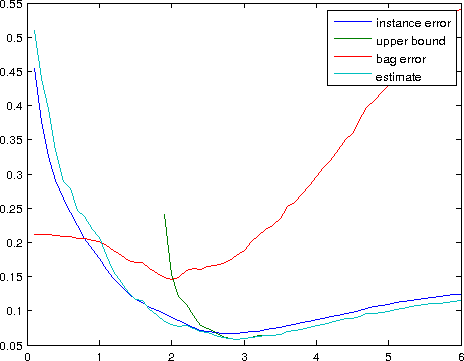
\includegraphics[height=63mm]{images/iid_03.png}
	\end{center}
	\caption{Error rates and bounds for dataset Gehler-iid. Top, center and bottom correspond to positive rates of 0.1, 0.2 and 0.3 respectively.
    We only look at low positive rates as in the i.i.d.\ case, high positive rates result in all bags being positive.
    See the text for details.}
	\figlabel{gehler_iid}
\end{figure}

\Figref{gehler_iid} compares the true instance error $e_I$, the bag error $e_B$, the estimate of $e_I$ using Theorem~\ref{equality}
and the bound of Theorem~\ref{iidbound} for datasets with different values of the positive instance rate.
The $x-axis$ shows different thresholds on estimated likelihood ratios, resulting in varying $h_0$.
It is apparent that the estimate of Theorem~\ref{equality} reflects the true error closely, with only little noise from the restricted
sample size. Note that the upper bound of Theorem~\ref{iidbound} is not defined everywhere. While it is quite tight when
$h_I^r \gg e_B$, it is not when $h_I^r \approx e_B$.


We also performed experiments using a dependent version of Gehler-org
with probabilistic constraints. Ten examples are drawn per bag and each example is positive with probability
of the fixed positive rate. We denote this dataset by Gehler-soft. In the original dataset, the number of positives and negatives in a positive bag
was deterministic, making the instances strongly dependent.

The new dataset Gehler-soft violates the i.i.d.\ assumption but satisfies the
restricted dependent assumption. \Figref{gehler_soft}
shows the values of the bound from Theorem~\ref{globalbound} and Theorem~\ref{lowerbound} compared to the
true instance error $e_I$ for different settings of the positive instance rate.
Inspecting the lower bound, which uses the same computation as the estimate in the i.i.d.\ case, we see that due to the limited
dataset size, the estimated lower bound actually lies above the actual error in some cases. On the other hand, for low positive
rates, the lower bound follows the true error quite closely.
The upper bound behaves quite different, being quite loose for low instance rates and thighter for high instance rates.
While the bounds on the true error might not always be very thight, it should be observed that they are clearly
non-trivial. This is surprising since we made only very general assumptions on the distribution of instances.

\begin{figure}[tbp]
	\begin{center}
		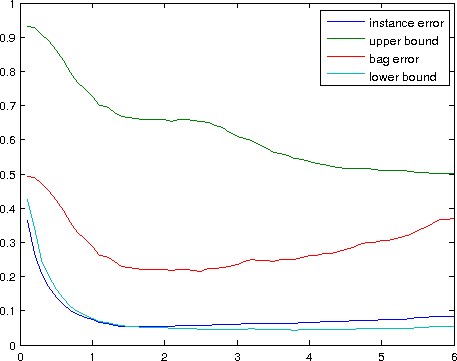
\includegraphics[height=63mm]{images/non_iid_02.png}
		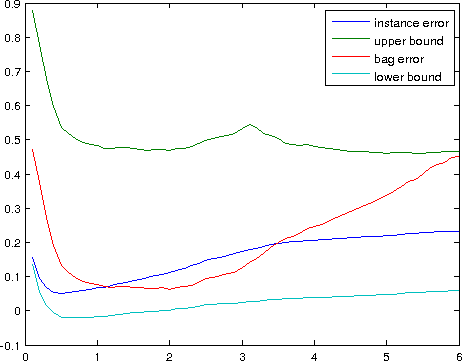
\includegraphics[height=63mm]{images/non_iid_05.png}
		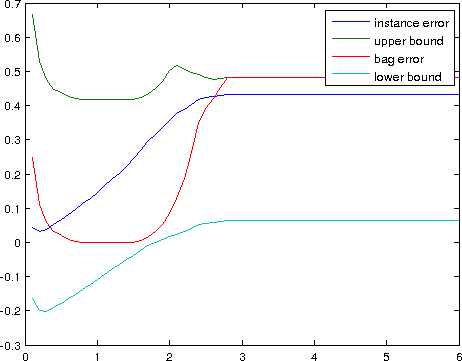
\includegraphics[height=63mm]{images/non_iid_09.png}
	\end{center}
	\caption{Error rates and bounds for dataset Gehler-soft. Top, center and bottom correspond to positive rates of 0.2, 0.5 and 0.9 respectively.
    See the text for details.}
	\figlabel{gehler_soft}
\end{figure}

\section{Conclusion}
We provided several bounds on instance prediction error in a multiple instance learning setting.
For the case that instances inside a bag are independent, we proved a strong upper bound on the error.
We showed that when bag labels are present, it is even possible to directly estimate the true instance error.

We introduced a restricted dependent setting for multiple instance learning, in which instances inside a bag
are only independent given an unobserved variable. We showed that without any further assumptions
on the distribution of this variable, it is possible to learn instance label prediction from bag labels
in this setting. We also provided upper and lower bounds on the instance error, given known bag labels
or an estimage of the bag error.
Empirical evaluation on a synthetic dataset with known dependen structure and known instance labels
showed that the bound are non-trivial and yield insight into the behavior of instance label errors.
We hope that this work establishes a basis for further research on instance label prediction
in multiple instance learning.

\section{Appendix}
\begin{lemma}\label{binarylemma}
Given two (dependent) binary random variables $x,y$:
\begin{equation}
p(x \neq y) = p(x=0) + p(y=0) - 2 p(x=0, y=0)
\end{equation}

\begin{proof}
\begin{align}
p(x \neq y) & = p(x=0, y=1) + p(x=1, y=0) \\
                &= p(x=0) - p(x=0, y=0)\\
                &  + p(y=0) - p(x=0, y=0) \\
                &= p(x=0) + p(y=0) -2 p(x=0, y=0)
\end{align}
\end{proof}
\end{lemma}

\begin{theorema}
Let all instances be independent. With bags $X$, instances $x$, true labels $y,Y$, $h_I$ any classifier
on instances and $h_B$ the resulting bag classifier, we have
\begin{align*}
   e_I = h_0 + p(y=0) - 2 \left (\frac{1}{2} ( h_0^r + p(y=0)^r - e_B) \right)^\frac{1}{r}
\end{align*}
\begin{proof}
    
\begin{align*}
e_B & = p(h_B(X) = 0) + p(Y=0) -2 p(h_B(X)=0, Y=0) \\\
&\text{using the lemma}\\
& = h_0^r + p(y=0)^r -2 p(h_I(x)=0, y=0)^r\\\
&\text{by independence}\\
& = h_0^r + p(y=0)^r -2 \left ( \frac{1}{2} (h_0 + p(y=0) - e_I) \right ) ^r \\
&\text{using Lemma~\ref{binarylemma} on }p(h_I(x)=0, y=0.
\end{align*}
Solving for $p(h_I(x)\neq y)$:
\begin{align*}
    & \left ( \frac{1}{2} (h_0 + p(y=0) - e_I )\right ) ^r = \frac{1}{2} \left ( h_0^r + p(y=0)^r - e_B \right )\\
    & \Rightarrow \frac{1}{2} (h_0 + p(y=0) - e_I)   = \left ( \frac{1}{2} \left ( h_0^r + p(y=0)^r - e_B \right ) \right )^\frac{1}{r}\\
    & \Rightarrow e_I   = h_0 + p(y=0) - 2 \left ( \frac{1}{2} \left ( h_0^r + p(y=0)^r - e_B \right ) \right )^\frac{1}{r}
\end{align*}
\end{proof}
\end{theorema}

\begin{corollarya}
If all instances are independent and bag classification is perfect, meaning $e_B=0$, then instance classification is also perfect ($e_I =0$).

\begin{proof}
Consider Theorem~\ref{basicthm}. If $e_B=0$ we have
\begin{align*}
p(h_I(x) \neq y) = h_0 + p(y=0) - 2 \left (\frac{1}{2} ( h_0^r + p(y=0)^r)) \right)^\frac{1}{r}
\end{align*}
By the convexity of the power function the right hand side of the equation is always greater or equal zero.
Since $e_I \geq 0$, both sides are equal zero.
\end{proof}
\end{corollarya}

\begin{theorema}
    If $h_0^r  \geq e_B$ and all instances are independent, we have
\begin{align}
    p(h_I(x)\neq y) \leq h_0 - \left ( h_0^r - e_B) \right ) ^ \frac{1}{r}
\end{align}
\begin{proof}
    Assume $h_0^r  \geq e_B$.
    From Theorem~\ref{basicthm} we have
\begin{align*}
   e_I &= h_0 + p(y=0) - 2 \left (\frac{1}{2} ( h_0^r + p(y=0)^r - e_B) \right)^\frac{1}{r}\\
   &\leq h_0 + p(y=0) - \left [( h_0^r + p(y=0)^r - e_B) \right]^\frac{1}{r}\\
   &- \left ( p(y=0)^r \right )^\frac{1}{r}\\
   &= h_0 - \left (( h_0^r + p(y=0)^r - e_B) \right)^\frac{1}{r}\\
\end{align*}
\end{proof}
\end{theorema}

\begin{theorema}
Let all instances be independent. Given $p(Y)$, the instance error $e_I$ can be calculated by
\begin{align}
    %\eqlabel{iid}
e_I = h_0 + p(Y=0)^\frac{1}{r} - 2 \left (\frac{1}{2} ( h_0^r + p(Y=0) - e_B) \right)^\frac{1}{r}.
\end{align}
\begin{proof}
    This follows from Theorem~\ref{basicthm} by using $p(Y=0)=p(y=0)^r$.
\end{proof}
\end{theorema}


\begin{theorema}
If the instance labels are independent inside a bag given a hidden cause, the instance
error $e_I$ has the following lower bound:
\begin{multline*}
e_I \geq h_0 + p(y=0) - \\
2 \left (\frac{1}{2} (p(h_B(X)=0) + p(Y=0) - e_B) \right)^\frac{1}{r}
\end{multline*}
\begin{proof}
    This follows from taking the expected value with respect to $Z$ of \eqref{conditioned} and using Jensen's
    inequality.
\end{proof}
\end{theorema}
